%%%%%%%%%%%%%%%%%%%%%%%%%%%%%%%%%%%%%%%
% PlushCV - One Page Two Column Resume
% LaTeX Template
% Version 1.0 (11/28/2021)
%
% Author:
% Shubham Mazumder (http://mazumder.me)
%
% Hacked together from:
% https://github.com/deedydas/Deedy-Resume
%
% IMPORTANT: THIS TEMPLATE NEEDS TO BE COMPILED WITH XeLaTeX
%
%
%%%%%%%%%%%%%%%%%%%%%%%%%%%%%%%%%%%%%%
%
% TODO:
% 1. Figure out a smoother way for the document to flow onto the next page.
% 3. Add more icon options
% 4. Fix hacky left alignment on contact line
% 5. Remove Hacky fix for awkward extra vertical space
%
%%%%%%%%%%%%%%%%%%%%%%%%%%%%%%%%%%%%%%
%
% CHANGELOG:
%
%%%%%%%%%%%%%%%%%%%%%%%%%%%%%%%%%%%%%%%
%
% Known Issues:
% 1. Overflows onto second page if any column's contents are more than the vertical limit.
%%%%%%%%%%%%%%%%%%%%%%%%%%%%%%%%%%%%%%
%%Icons:
%%Main: https://icons8.com/icons/carbon-copy
%%%%%%%%%%%%%%%%%%%%%%%%%%%%%%%%%%

\documentclass[]{plushcv}
\usepackage{fancyhdr}
\pagestyle{fancy}
\fancyhf{}
\begin{document}

%%%%%%%%%%%%%%%%%%%%%%%%%%%%%%%%%%%%%%
%
%     TITLE NAME
%
%%%%%%%%%%%%%%%%%%%%%%%%%%%%%%%%%%%%%%


\namesection{Haroune}{Mohammedi}{Mid-Level Software Engineer - Data Engineer\hfill\smash{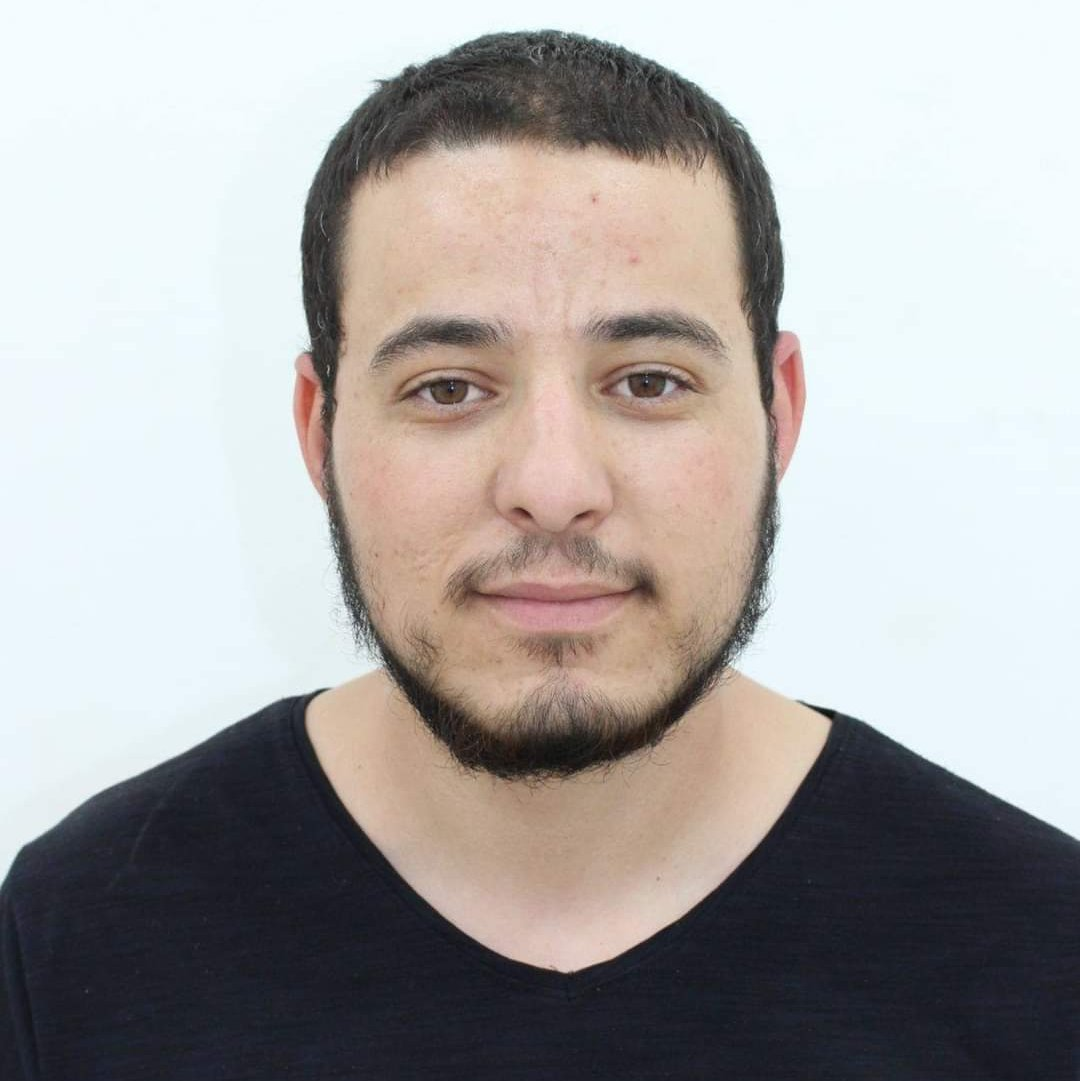
\includegraphics[width=3cm]{me.jpg}}}{\small\contactline{\href{https://www.mazumder.me}{mazumder.me}}{\href{https://www.github.com/mohammedi-haroune}{mohammedi-haroune}}{\href{https://www.linkedin.com/in/haroune-mohammedi-3b3836170/}{haroune-mohammedi}}{\href{mailto:mohammedi.haroun@gmail.com}{mohammedi.haroun@gmail.com}}{\href{tel:+213698056800}{+213698056800}}}

% \namesection{Firstname}{Lastname}{Full Stack Software Engineer}{\contactline{\href{https://www.mazumder.me}{mazumder.me}}{\href{https://www.github.com/sansquoi}{sansquoi}}{\href{https://www.linkedin.com/mazumders}{mazumders}}{\href{mailto:shubham.mazumder@gmail.com}{first.last@email.com}}{\href{tel:+1999999999}{9999999999}}}

%%%%%%%%%%%%%%%%%%%%%%%%%%%%%%%%%%%%%%
%
%     COLUMN ONE
%
%%%%%%%%%%%%%%%%%%%%%%%%%%%%%%%%%%%%%%

\begin{minipage}[t]{0.70\textwidth}


%%%%%%%%%%%%%%%%%%%%%%%%%%%%%%%%%%%%%%
%     EXPERIENCE
%%%%%%%%%%%%%%%%%%%%%%%%%%%%%%%%%%%%%%

\section{Experience}

\runsubsection{BigMama Technologies}
\descript{| Software Engineer (Python) }
\location{July 2019 – Present | Algiers, Algeria}
\vspace{\topsep} % Hacky fix for awkward extra vertical space
\begin{tightemize}
\sectionsep
\item Core developper of https://iko.ai, a machine learning platform that offers real-time collaborative notebooks to train, track, package, deploy, and monitor machine learning models.
\item Analyze requirements then desing and build software to solve the problem.
\item Compare open-source solutions, synthesiz, the integrate the best solution of our needs.
\item Aquire a business oriented perspective of Softawre Engineering and leart to put value ahead of implementation details
\item Communicate ideas effectively in Gitlab issues, work on a fully remote environment for more than a year
\item Backend developpement with Flask
\item Write Python applications that deploy workloads in Kuberentes
\end{tightemize}
\sectionsep

\runsubsection{BigMama Technologies}
\descript{| Data Engineer (Scala) }
\location{September 2017 – Juin 2019 | Algiers, Algeria}
\begin{tightemize}
\sectionsep
\item Built and deployed a data-intensive application on top off akka, spark, kafka, elasticsearch and firebase, focusing on high-availability, fault
tolerance, and scalability.
\item Developed an internal sdk using scala for integrating different dynamic parts of our stack (firebase, kafka, akka ..ect), focusing on maintenabily
and extensiblity
\item Contributed to the design of many complex applications based on actor model and designed to be distrubuted, highly-scalable and fault-tolent.
\item Provisioned Ansible recipes for internal infromation systems setup (Gitlab, Apt Mirror, SFTP, 2FA Authentitcation
\end{tightemize}
\sectionsep

\runsubsection{IB-Network}
\descript{| Software Engineer Intern }
\location{May 2016 - July 2016 | Algiers, Algeria}
\begin{tightemize}
\sectionsep
\item Desinged and Build a management application
\item Working under a responsable, manage deadlines.
\item Getting my hands on how clients should be handled.
\end{tightemize}
\sectionsep


%%%%%%%%%%%%%%%%%%%%%%%%%%%%%%%%%%%%%%
%     Projects
%%%%%%%%%%%%%%%%%%%%%%%%%%%%%%%%%%%%%%

\section{Projects}

\runsubsection{Domain Specific Language for Raisnoning Systems}
\descript{| Scala}
\location{2018 | University project}
\begin{tightemize}
\item Fulfill my curiosity and explore how to make DLSs in Scala
\end{tightemize}
\sectionsep

\runsubsection{Video player controlled by hand gestures}
\descript{| Scala, Akka}
\location{2018 | University project}
\begin{tightemize}
\item Asynchrous and recative JavaFx based app
\item Actor model architecture using Akka and Akka remote
\item Hand gesture detection neural network model trained with Keras
\end{tightemize}
\sectionsep

%%%%%%%%%%%%%%%%%%%%%%%%%%%%%%%%%%%%%%
%     AWARDS
%%%%%%%%%%%%%%%%%%%%%%%%%%%%%%%%%%%%%%

% \section{Awards}
% \begin{tabular}{rll}
% 2018	     & Winner, Algerian Collegiate Programming Contest (ALCPC)\\
% \\
% \end{tabular}
% \sectionsep
%%%%%%%%%%%%%%%%%%%%%%%%%%%%%%%%%%%%%%
%
%     COLUMN TWO
%
%%%%%%%%%%%%%%%%%%%%%%%%%%%%%%%%%%%%%%

\end{minipage}
\hfill
\begin{minipage}[t]{0.25\textwidth}

%%%%%%%%%%%%%%%%%%%%%%%%%%%%%%%%%%%%%%
%     SKILLS
%%%%%%%%%%%%%%%%%%%%%%%%%%%%%%%%%%%%%%

\section{Skills}
\subsection{Programming}
\sectionsep
\location{Proficient:}
Python \textbullet{} Flask  \\
\sectionsep
\location{Experienced:}
Scala \textbullet{} Akka \textbullet{}  Cats \textbullet{} HTML/CSS/JS  \\
\sectionsep
\location{Familiar:}
TypeScript \textbullet{}  Shell \textbullet{} Vuejs \textbullet{} Spark \\
\sectionsep
\sectionsep
% \subsection{Libraries/Frameworks}
% \sectionsep
% Akka \textbullet{} cats \textbullet{} Flask \textbullet{} Vuejs \\
% \sectionsep
\sectionsep
\subsection{Tools/Platforms}
\sectionsep
Git \textbullet{} Docker \textbullet{} Kubernetes \\

\sectionsep

%%%%%%%%%%%%%%%%%%%%%%%%%%%%%%%%%%%%%%
%     EDUCATION
%%%%%%%%%%%%%%%%%%%%%%%%%%%%%%%%%%%%%%

\section{Education}
\subsection{University of Houari Boumedien Bab Ezzouar}
\descript{PhD in Computer Science}
\location{Sep 2019 - Present | Algiers, Algeria}
Data science, Multicloud \\
% \location{ Cum. GPA: 3.85 / 4.0 }

\subsection{University of Houari Boumedien Bab Ezzouar}
\descript{Master's in Computer Science}
\location{Sep 2017 - June 2019 | Algiers, Algeria}
% School of Computing \\
% \location{ Cum. GPA: 3.85 / 4.0 }

\sectionsep
\subsection{University of Houari Boumedien Bab Ezzouar}
\descript{Bachelor's in Computer Science
\\and Engineering}
\location{Sep 2014 - June 2017 | Algiers, Algeria}
% School of Computing \\
% \location{ Cum. GPA: 3.7 / 4.0 }
\sectionsep

% %%%%%%%%%%%%%%%%%%%%%%%%%%%%%%%%%%%%%%
% %     REFERENCES
% %%%%%%%%%%%%%%%%%%%%%%%%%%%%%%%%%%%%%%

\section{References}

\href{https://www.linkedin.com/in/pr-youcef-aklouf-08485729/}{\textbf{Pr. Youcef Aklouf}}, Professor at USTHB | R\&D Manager at KBMC consulting, France
\\
\begingroup
\setbox0=\hbox{

\includegraphics[scale=0.1,trim={0 1cm 0cm 0cm}]{icons/main/mail.png}\hspace{0.3cm} yaklouf@yahoo.fr
}
\parbox{\wd0}{\box0}
\endgroup

\sectionsep
\href{https://www.linkedin.com/in/adlane-kadri-788b66138/}{\textbf{Adlane Kadri}, Software Engineer, Innoscape, France}
\begingroup
\setbox0=\hbox{

\includegraphics[scale=0.1,trim={0 1cm 0cm 0cm}]{icons/main/mail.png}\hspace{0.3cm} adlan68@live.fr
}
\parbox{\wd0}{\box0}
\endgroup
% \begingroup
% \setbox0=\hbox{
% 
\includegraphics[scale=0.1,trim={0 1.25cm -0.4cm 0cm}]{icons/main/phone.png}\hspace{0.3cm}+19999999999
% }
% \parbox{\wd0}{\box0}\endgroup
\\

\sectionsep
\href{https://www.linkedin.com/in/yahiabattach/}{\textbf{Yahia Bettach}}, Software Developer, Resel, Saudi Arabie
\\
\begingroup
\setbox0=\hbox{

\includegraphics[scale=0.1,trim={0 1cm 0cm 0cm}]{icons/main/mail.png}\hspace{0.3cm} battachyahia@hotmail.com
}
\parbox{\wd0}{\box0}
\endgroup
% \begingroup
% \setbox0=\hbox{
% 
\includegraphics[scale=0.1,trim={0 1.25cm -0.4cm 0cm}]{icons/main/phone.png}\hspace{0.3cm}+19999999999
% }
% \parbox{\wd0}{\box0}\endgroup
\\
%%%%%%%%%%%%%%%%%%%%%%%%%%%%%%%%%%%%%%
%     COURSEWORK
%%%%%%%%%%%%%%%%%%%%%%%%%%%%%%%%%%%%%%

% \section{Coursework}

% \subsection{Graduate}
% Graduate Algorithms \textbullet{}\\
% Advanced Computer Architecture \textbullet{}\\
% Operating Systems \textbullet{}\\
% Artificial Intelligence \textbullet{}\\
% Visualization For Scientific Data \\
% \sectionsep

% \subsection{Undergraduate}

% Database Management Systems \textbullet{}\\
% Object Oriented Analysis and Design \textbullet{}\\
% Artificial Intelligence and Expert Systems \textbullet{}\\
% Scripting Languages and Web Tech \textbullet{}\\
% Software Engineering \\

\end{minipage}
\end{document}  \documentclass[]{article}
